\documentclass[conference]{IEEEtran}
\usepackage{graphicx}
\usepackage[strings]{underscore}
\usepackage{biblatex}
\usepackage{xurl}

%Title
\title{Contour Detection Algorithms}
\author{
    \IEEEauthorblockN{Sotheanith Sok}
    \IEEEauthorblockA{
        Department of Engineering\\ 
        California State University of Long Beach\\
        Sotheanith.Sok@student.csulb.edu
    }
}
\date{October 3 2021}

\addbibresource {refs.bib}

\begin{document}

\maketitle

\section{Introduction}
In computer vision, contour detection algorithms are used to find a boundary of an image and it is usually the first preprocessing step prior to other processes such as foreground extraction, image segmentation, object detection, and so on. There are many contour detection algorithms but the two most popular algorithms are Square Tracing Algorithm and More Neighborhood Algorithm. This paper will explore how these two algorithms work, their advantages, and their limitations.

\section{Square Tracing Algorithm}

\begin{figure}[!htb]
    \centering
    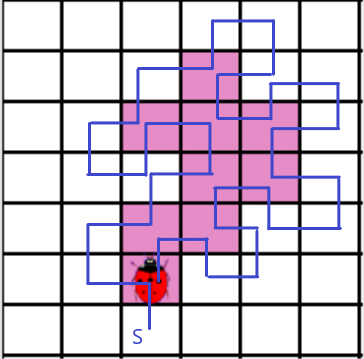
\includegraphics[scale = 0.5]{fig1.png}
    \caption{Square Tracing Algorithm demonstration. S indicates the starting position and blue lines indicate the algorithm's path \cite{sta:2000}.}
\end{figure}

Square Tracing Algorithm is one of the first contour detection algorithms that remains in use today. The algorithm assumes that an image is divided into two regions: black pixels for the object and white pixels for the background. At its fundamental level, the algorithm starts by picking a black pixel and marking it as the starting pixel. Then, the algorithm will decide on its next pixel based on the current pixel and how it was entered(orientation). If the current pixel is black, the next pixel will be located 90° from the current pixel's orientation in the counter-clockwise direction. But, if the current pixel is white, the next pixel will be located 90° from the current pixel's orientation in the clockwise direction. These steps are repeated until the starting pixel is reached again and the algorithm is terminated.

\begin{figure}[!htb]
    \centering
    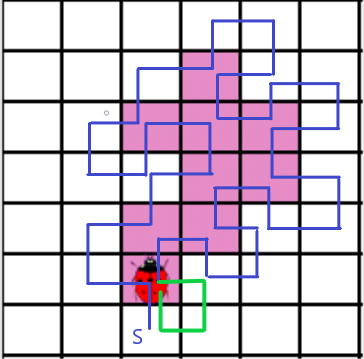
\includegraphics[scale = 0.5]{fig2.png}
    \caption{Square Tracing Algorithm with Jacob's stopping criterion demonstration. S indicates the starting position, blue lines indicate the algorithm's path, and green lines indicate the extra path from Jaco's stopping criterion \cite{sta:2000}.}
\end{figure}

Unfortunately, terminating the algorithm after it visited the starting pixel twice is a major reason behind the algorithm's poor performance on patterns that occur frequently in real life. As such, in order to overcome such limitation, two new stopping criteria are suggested. The first alternative stopping criterion is the simplest and it increases the number of visit of the starting pixel before the algorithm terminated to more than 2. The second alternative stopping criterion, suggested by Jacob Eliosoff, is modifying the stopping condition such that the starting pixel's orientation is factored in. Simply put, if the algorithm entered the starting pixel from the westward direction, the algorithm only terminated if it visited the starting pixel again from the same direction.

\begin{figure}[!htb]
    \centering
    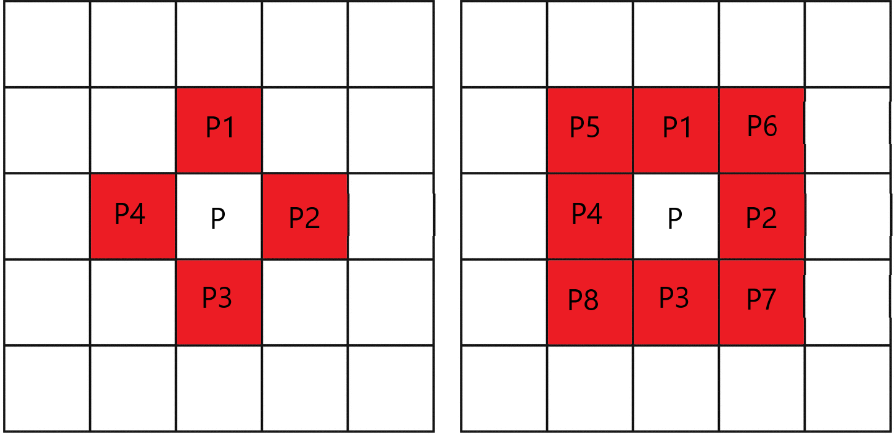
\includegraphics[scale = 0.3]{fig3.png}
    \caption{The left figure has a 4-connected pattern and the right figure has an 8-connected pattern \cite{gct:2010, dc:2000}.}
\end{figure}

In general, delaying the algorithm's termination tends to improve the overall performance but it does not address another limitation. A pixel's connection pattern can be classified into two categories: 4-connected and 8-connected. To start with, a pixel is said to have a 4-connected pattern if it shares at least one side with another pixel of the same color. Thus, a pixel is said to have an 8-connected pattern if it has a 4-connected pattern or if it shares a vertex with another pixel of the same color. According to \cite{sta:2000}, Square Tracing Algorithm using Jacob's stopping criterion will guarantee to fully trace the contour of an object without visiting the starting pixel more than twice if both regions of an image are not disconnected and every pixel has a 4-connected pattern.

\section{Moore Neighborhood Algorithm}

\begin{figure}[!htb]
    \centering
    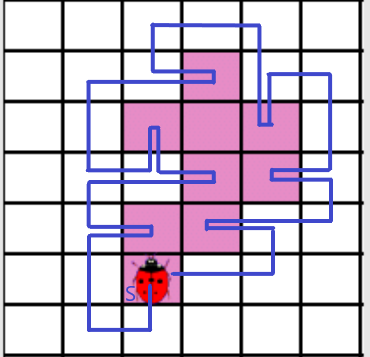
\includegraphics[scale = 0.5]{fig4.png}
    \caption{Moore Neighborhood Algorithm demonstration. S indicates the starting position and blue lines indicate the algorithm's path \cite{mnt:2000}.}
\end{figure}

Moore Neighborhood Algorithm is another contour detection algorithm and it remains popular today due to its simplicity and its effectiveness. Similar to Square Tracing Algorithm, this algorithm assumes that an image is divided into two regions: black pixels for the object and white pixels for the background. The algorithm starts by finding a black pixel and marks it as the starting pixel and the current pixel. Then, the algorithm will check all neighboring pixels of the current pixel to find a black pixel in a clockwise direction. Once a black pixel is found, it will be set as the current pixel and the algorithm will check all of its neighboring pixels starting from the latest white pixel of the previous current pixel. These steps are repeated until the starting pixel is visited again and the algorithm is terminated.

\begin{figure}[!htb]
    \centering
    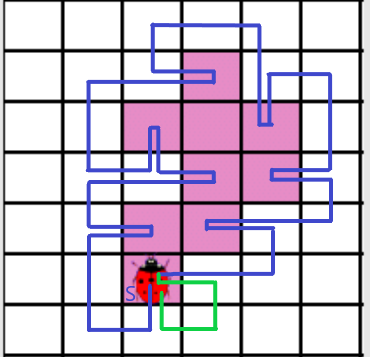
\includegraphics[scale = 0.5]{fig5.png}
    \caption{Square Tracing Algorithm with Jacob's stopping criterion demonstration. S indicates the starting position, blue lines indicate the algorithm's path, and green lines indicate the extra path from Jaco's stopping criterion \cite{mnt:2000}.}
\end{figure}

Unfortunately, similar to Square Tracing Algorithm, setting the termination condition as visiting the starting pixel twice will hinder the performance of Moore Neighborhood Algorithm. As such, the two alternative stopping criteria described above can also be applied to this algorithm and they will improve the performance of the algorithm. Interestingly, according to \cite{mnt:2000}, combining Moore Neighborhood Algorithm with Jacob's stopping criterion will ensure that the algorithm can find contour for any patterns including 4-connected patterns, 8-connected patterns, or a mix of both because the algorithm will check all neighboring pixels of a pixel.

\section{Final Thought}
Square Tracing Algorithm and Moore Neighborhood Algorithm are good contour detection algorithms due to their simplicity and their effectiveness. However, it is recommended that Jacob's stopping criterion should be used with both algorithms as delaying the termination condition will generally improve algorithms' performance. Furthermore, as stated previously, Square Tracing Algorithm should only be used on an image that contains only 4-connected patterns and all regions are not disconnected to ensure its optimal performance. For all images, Moore Neighborhood Algorithm with Jacob's stopping criteria is the recommended counter detection algorithm as it will be able to detect counter for any patterns.

\printbibliography

\end{document}
